\chapter{Integer Programming}
\label{cha:integer_programming}
This chapter focuses on some preliminaries around integer
programming---which is a subarea of (mathematical) optimization.
In that context we introduce three common optimization problems which
can be solved using integer programming: SAT, Vertex Cover, and
Independent Set. They are discussed later within this thesis
(\cref{cha:triangulations,cha:mmlt}) in association with the
\gls{MMLT} problem.

An integer program is basically a problem description as a system
of (in-)equations involving only variables with integer values. As
an addition there can be an objective function for modeling
optimization problems. Throughout this thesis, we assume that every
integer program has only linear (in-)equations which is referred to as
a \emph{linear integer program}.

\begin{definition}[(Linear) \gls{IP}]
  An \gls{IP} is a system of integer variables
  \(x \in \gls{Z}^n (n \in \gls{N})\)
  with a set of constraints on them
  and optionally an objective function. 
  We consider only the case
  where the constraints are linear with respect to \(x\).
\end{definition}

A natural standardized way of formulating (linear) \gls{IP}[s] is the 
so called \emph{canonical form.} It combines the coefficients of the
variable vector \(x \in \gls{Z}^n (n \in \gls{N})\)
for all \(m \in \gls{N}\) (in-)equations
in a matrix \(A \in \gls{Z}^{m \times n}\), 
all constant terms are
summed up to a vector \(b \in \gls{Z}^m\), and the objective function is represented
as a multiplication of the variables \(x\) and a constant target
vector \(c \in \gls{Z}^n\). For readability, we slightly modify the canonical form,
e.g. by allowing sums.

\begin{problem}[\gls{IP} in canonical form \cite{combinatorial_optimization}]
  \[
  \begin{array}{lll}
    \begin{alignedat}{2}
      &\text{maximize } & c^Tx \\
      &\text{subject to } & Ax &\leq b \\
      && x &\geq 0 \\
      && x &\in \gls{Z}^n
    \end{alignedat}
    & \text{\hspace{2em}or\hspace{2em}} &
    \begin{alignedat}{2}
      &\text{minimize } & c^Tx \\
      &\text{subject to } & Ax &\geq b \\
      && x &\leq 0 \\
      && x &\in \gls{Z}^n
    \end{alignedat}
  \end{array}
  \]
  (\(\leq\) and \(\geq\) here denote the row-wise comparison
  of two vectors)
\end{problem}

Even though the structure of \gls{IP}[s] looks very simple, it is a
long known fact that solving them is not easy. Nevertheless they come
in useful for various optimization problems---especially because there
are many practical applications involving only integers. A common
strategy to simplify the problem is leaving out the integrity
restriction for retrieving bounds of the optimal solution.

\begin{theorem}
  Solving \gls{IP}[s] is NP-hard.
  \begin{proof}
  Even the special case where there is no objective function, only
  binary variables, and only equality constraints is NP-complete
  \cite{karp_np_complete}. 
  Therefore the more general problem is NP-hard.
  \end{proof}
\end{theorem}

\section{SAT}
The (boolean) satisfiability problem (SAT) asks for a variable
assignment which fulfills a logical term. It was the first problem to
be proven NP-complete \cite{np_complete} and has since been a common
choice for NP-hardness proofs---many times even more restricted such
as the 3-SAT problem which allows only for three variables in each
``sub-term'' (clause).

\begin{problem}[3-SAT]
  \label{prob:3SAT}\hfill
  \begin{labeling}{\hspace{4em}}
    \item[\textbf{Given:}]
      Set of boolean literals \(X\), a formula in conjunctive 
      normal form consisting of clauses \(C\) each involving 
      exactly three literals (or their negations)
    \item[\textbf{Sought:}]
      An assignment for \(X\) which lets all clauses in \(C\) evaluate
      to ``true''
  \end{labeling}
\end{problem}

Shortly after the concept of NP-completeness was introduced in
\cite{np_complete}, Richard Karp applied the idea to several other
well-known problems \cite{karp_np_complete}. One of them was the
3-SAT problem which has more structure than the general boolean
satisfiability problem and is therefore easier to embed into
constructive NP-hardness or NP-completeness proofs.

\begin{theorem}[NP-completeness of 3-SAT]
  \Cref{prob:3SAT} is NP-complete.~\cite[Satisfiability with at most %
  3 Literals per Clause]{karp_np_complete}
\end{theorem}

As already mentioned earlier, the 3-SAT problem can be formulated as
an \gls{IP}. This easily confirms the NP-hardness of solving
\gls{IP}[s]. Additionally it allows for applying \gls{IP} solvers 
(such as CPLEX, see also \cref{sec:cplex}) to 3-SAT problems. Usually
however, SAT solvers are used which take advantage of the problem
structure better and have therefore less overhead.

\begin{problem}[\gls{IP} formulation of 3-SAT]
  \begin{alignat*}{3}
    &(\text{minimize } & 0^Tx) \\
    &\text{subject to } & \forall c \in C : &~
    & \sum\limits_{x_i \in c} x_i + \sum\limits_{\lnot x_i \in c} (1 - x_i) &= 1 \\
    && \forall x_i \in X : &~& x_i &\in \{0,1\}
  \end{alignat*}
  (\(x_i \in c\) (or \(\lnot x_i \in c\)) herein denotes that
  \(x_i\) (or \(\lnot x_i\)) is part of the clause \(c\))
\end{problem}

For geometric and graph problems an even more restricted class of
3-SAT problem has been established, the \emph{Planar 3-SAT}. It asks
for the connection graph of all clauses and their variables to be
embeddable in the plane.

\begin{problem}[Planar 3-SAT]
  \label{prob:planar_3SAT}
  An instance of the 3-SAT problem with literals \(X\) and
  clauses \(C\) which can be represented by a planar graph
  \(G = (V,E)\) such that
  \begin{alignat*}{1}
    V &= \{v : v \in X \cup C\} \\
    E &= \{ \{x, c\} :
      x \in X,~
      c \in C,~
      (x \in c) \lor (\lnot x \in c)
    \}
  \end{alignat*}
\end{problem}

\Cref{fig:example_planar_3SAT} shows an example of a 3-SAT instance
with a planar variable-clause-connection graph. There is a vertex for
every clause (mint colored squares) and every variable (red circles)
and edges in between if a variable (or its negation) is part of a
clause.

\begin{figure}[ht]
  \centering
  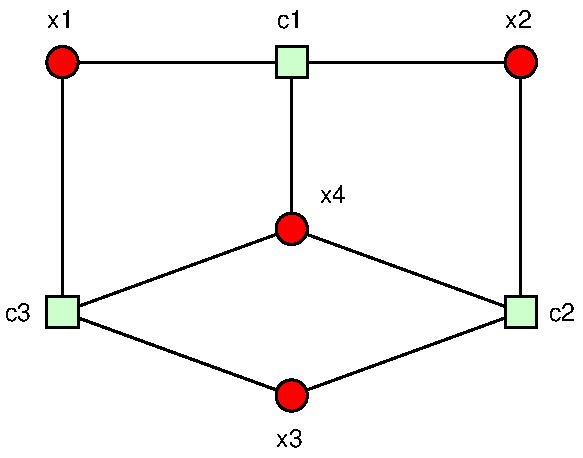
\includegraphics[width=0.5\textwidth]{img/example_planar_3SAT.pdf}
  \caption{\label{fig:example_planar_3SAT}Example of a Planar 3SAT %
    instance which represents the term \(%
      \protect\underbrace{(x_1 \lor x_2 \lor x_4)}_{c_1}\land%
      \protect\underbrace{(\lnot x_2 \lor x_3 \lor \lnot x_4)}_{c_2}\land%
      \protect\underbrace{(x_1 \lor \lnot x_3 \lor \lnot x_4)}_{c_3}%
    \)}
\end{figure}

It was shown that even this restricted class of satisfiability
problems is NP-complete. That way problems can be proven to be
NP-hard in the plane without having to deal with intersections. This
result can then be used for higher dimensions (usually, problems
become harder to solve if they are elevated to higher dimensions).

\begin{theorem}[NP-completeness of Planar 3-SAT]
  \Cref{prob:planar_3SAT} is still NP-complete.~\cite{planar_3SAT}
\end{theorem}

\section{Vertex Cover}
\label{sec:vertex_cover}
Another problem in the collection of \cite{karp_np_complete} is
\emph{Vertex Cover} which aims to cover (all) edges of a graph by
their incident vertices. It is closely related to other graph problems
such as Edge Cover, Clique, Independent Set
(see \cref{sec:independent_set}), Coloring, and the more general Set
Cover.

\begin{definition}[Vertex Cover]
  \label{def:vertex_cover}
  Given an undirected graph \(G=(V,E)\), a Vertex Cover
  \(\gls{VC} \subseteq V\) for \(G\) is a vertex set such that
  every edge \(e \in E\) is incident to at least one vertex
  \(v \in \gls{VC}\):
  \[ \forall e \in E: \exists v \in \gls{VC}: v \in e \]
\end{definition}

A trivial Vertex Cover of any graph \(G=(V,E)\) would be the complete
vertex set \(V\). In general, such a Vertex Cover is not useful but
one asks for the covering vertex set to be minimal (roughly speaking
without unnecessary vertices).

\begin{definition}[Minimal Vertex Cover]
  A Vertex Cover \gls{VC} for an undirected graph
  \(G=(V,E)\) is minimal if there is no vertex
  \(v \in \gls{VC}\) such that
  \(\gls{VC} \setminus \{v\}\) remains a Vertex Cover.
\end{definition}

Still, \emph{any} Minimal Vertex Cover is not always wanted as it
needs not be unique---hence there can be a much smaller covering
vertex set. An extreme example is a star-shaped graph where one vertex
can cover all edges but the set of all other vertices would also be
minimal. Therefore we distinguish between a Minimal Vertex Cover and
a \emph{Minimum} Vertex Cover, i.e. a smallest possible one. 
\Cref{fig:example_vertex_cover} shows the difference between Minimal
and Minimum Vertex Cover by example.

\begin{definition}[Minimum Vertex Cover]
  A Vertex Cover \gls{VC} for an undirected graph
  \(G=(V,E)\) is minimum if there is no other Vertex Cover
  \(\gls{VC}[']\) for \(G\) which has fewer vertices:
  \[
    \forall~V_{\text{cover}}'\text{ Vertex Cover} :
    |\gls{VC}| \leq |\gls{VC}[']|
  \]
\end{definition}

\begin{figure}[ht]
  \centering
  \begin{subfigure}{0.25\textwidth}
    \centering
    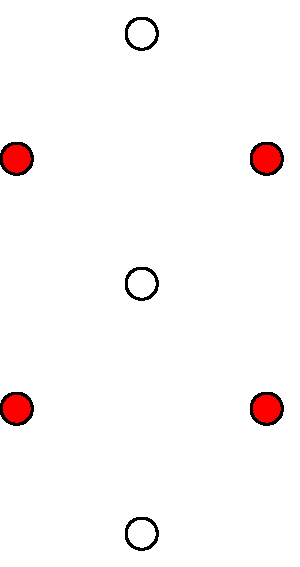
\includegraphics[width=\textwidth]{img/example_minimal_vertex_cover.pdf}
    \caption{Minimal}
  \end{subfigure}
  \hspace{2em}
  \VRule
  \hspace{2em}
  \begin{subfigure}{0.25\textwidth}
    \centering
    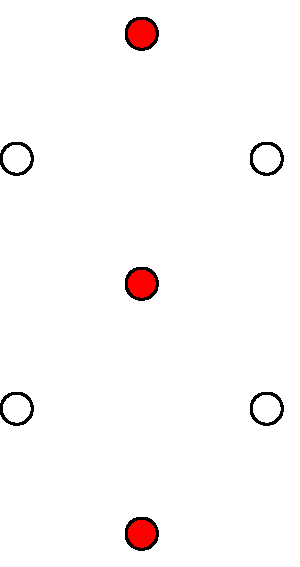
\includegraphics[width=\textwidth]{img/example_minimum_vertex_cover.pdf}
    \caption{Minimum}
  \end{subfigure}
  \caption{\label{fig:example_vertex_cover}%
    Example of Minimal vs. Minimum Vertex Cover, covering vertices %
    in red
  }
\end{figure}

The \gls{IP} formulation of Minimum Vertex Cover can be directly
deduced from the definition: We minimize the number of covering
vertices such that for every edge at least one vertex is selected. The
optimal vertex set \(\gls{VC}\) can then be retrieved from the
\gls{IP} solution vector by just collecting all selected vertices:
\( \gls{VC} = \{v \in V \land x_v = 1\} \)

\begin{problem}[\gls{IP} Formulation of Minimum Vertex Cover]
  \begin{alignat*}{3}
    &\text{minimize } & \sum\limits_{v \in V} x_v \\
    &\text{subject to } & \forall \{v,w\} \in E : &~& x_v + x_w &\geq 1 \\
    && \forall v \in V : &~& x_v &\in \{0,1\}
  \end{alignat*}
\end{problem}

What follows is that the Minimum Vertex Cover is also NP-complete
because it is a subset of the Set Cover
problem~\cite{karp_np_complete} and clearly lies in NP as it can be
(polynomially) reduced to solving \gls{IP}[s].

\begin{theorem}[NP-completeness of Minimum Vertex Cover]
  \label{thm:minimum_vertex_cover_complexity}
  Minimum Vertex Cover is NP-complete.~\cite{karp_np_complete}
\end{theorem}

We now introduce the class of \gls{wcover} graphs which we will need
in \cref{cha:triangulations}. They combine all graphs in which there
is no difference between Minimal and Minimum Vertex Cover. Minimal
Vertex Covers can be calculated with significant less effort (i.e. 
in polynomial time) than Minimum Vertex Covers (e.g. by just
iteratively removing vertices from the set until it would destroy the
covering property). This leads to Minimum Vertex Cover being solvable
in polynomial time for \gls{wcover} graphs.

A subset of \gls{wcover} graphs are connected bipartite graphs
\(G=(A \cup B,E \subseteq A \times B)\) with both vertex sets having
the same size: \(|A|=|B|\). Either one of \(A\) and \(B\) is a Minimal
and a Minimum Vertex Cover for \(G\). Clearly this graph class is not
empty which already implies that the class of \gls{wcover} graph is
not empty either.

\begin{definition}[\Gls{wcover} Graph]
  \label{def:well_covered}
  An undirected graph \(G=(V,E)\) is \gls{wcover} iff every Minimal
  Vertex Cover for \(G\) is also a Minimum Vertex Cover for \(G\).
  \cite{graph_well_covered}
\end{definition}

As a logical consequence of \cref{def:well_covered}, every two vertex 
sets which are a Minimal Vertex Cover for a \gls{wcover} graph \(G\)
have the same size. If one of them had more vertices than the other
one, it could not have been a Minimum Vertex Cover for \(G\)---which
contradicts \(G\) being \gls{wcover}.

\begin{theorem}
  \label{thm:well_covered_vertex_cover}
  In a \gls{wcover} graph, all Minimal Vertex Covers have the same
  cardinality. \cite{graph_well_covered}
\end{theorem}

\section{Independent Set}
\label{sec:independent_set}
Another prominent graph problem is the \emph{Independent Set} which
asks for a vertex set that is ``independent'', meaning that no two
vertices are adjacent. It can be seen as the counter part of Vertex
Cover (see \cref{sec:vertex_cover}) because it requires \emph{at most}
one vertex for every edge while Vertex Cover demands \emph{at least}
one vertex for every edge. We consider this connection in 
\cref{thm:independent_set_vertex_cover}.

\begin{definition}[Independent Set]
  \label{def:independent_set}
  Given an undirected graph \(G=(V,E)\), an independent set
  \(\gls{IS} \subseteq V\) is a vertex set such that no two
  vertices \(v,w \in \gls{IS}\) are incident to the same edge 
  \(\{v,w\} \in E\):
  \[
    \forall v \in \gls{IS}:
    \forall \{v,w\} \in E:
    w \not\in \gls{IS}
  \]
\end{definition}

Again we can find a trivial Independent Set for every graph in
constant time: the empty set. However, similar to Vertex Cover one 
usually asks for a ``large'' Independent Set as defined below:

\begin{definition}[Maximal/Maximum Independent Set]
  \label{def:max_independent_set}
  For an undirected graph \(G=(V,E)\), an independent set
  \(\gls{IS}\subseteq V\) is maximal if there is no vertex
  \(v \in V\setminus \gls{IS}\) such that
  \(\gls{IS} \cup \{v\}\) remains an independent set. It is
  maximum if there is no independent set \(\gls{IS}'\) with
  larger cardinality.
\end{definition}

The \gls{IP} for Maximum Independent Set maximizes the number of 
selected vertices such that for every edge only one of the incident 
vertices is selected. Analogous to the \gls{IP} formulation of Minimum
Vertex Cover, the optimal \gls{IS} solution can directly be retrieved 
from the \gls{IP} solution:
\( \gls{IP} = \{v \in V : x_v = 1\} \)

\begin{problem}[\gls{IP} Formulation of Maximum Independent Set]
  \begin{alignat*}{3}
    &\text{maximize } & \sum\limits_{v \in V} x_v \\
    &\text{subject to } & \forall \{v,w\} \in E : &~& x_v + x_w &\leq 1 \\
    && \forall v \in V : &~& x_v &\in \{0,1\}
  \end{alignat*}
\end{problem}

We already mentioned the close connection between Vertex Cover and
Independent Set earlier. Note that in \cref{fig:example_vertex_cover}
the Minimal Vertex Cover is a Maximum Independent Set and the Minimum
Vertex Cover a Maximal Independent Set. From the \gls{IP} formulations
 it can also been seen that the problems behave the opposite way:

\begin{theorem}[Independent Set and Vertex Cover]
  \label{thm:independent_set_vertex_cover}
  For an undirected graph \(G=(V,E)\), \(\gls{IS} \subseteq V\)
  is a Maximum Independent Set if and only if
  \(\gls{VC} = V \setminus \gls{IS}\)
  is a Minimum Vertex Cover.
  \begin{proof}
  Let \gls{VC} be a Vertex Cover for \(G\). 
  \begin{alignat*}{1}
    \forall e \in E : \exists v \in \gls{VC} : v \in e
    &\iff \forall \{v,w\} \in E :
      v \in \gls{VC} \lor w \in \gls{VC} \\
    &\iff \forall \{v, w\} \in E :
      \lnot(v \not\in \gls{VC} \land w \not\in \gls{VC}) \\
    &\iff \forall \{v, w\} \in E :
      \lnot(v \in (V \setminus \gls{VC})
        \land w \in (V \setminus \gls{VC})) \\
    &\iff \forall v \in (V \setminus \gls{VC}) :
      \forall \{v, w\} \in E :
      w \not\in (V \setminus \gls{VC}) \\
    &\iff (V \setminus \gls{VC}) \text{ independent set}
  \end{alignat*}
  
  Assume \gls{VC} is a Minimum Vertex Cover for \(G\) and the
  independent set \(\gls{IS} = V \setminus \gls{VC}\) is not maximum.
  Then there is an independent \(\gls{IS}['] \subseteq V\) with
  \(|\gls{IS}| < |\gls{IS}[']|\). But then for the Vertex Cover
  \(\gls{VC}['] = V \setminus \gls{IS}[']\) the following holds:
  \(|\gls{VC}[']| < |\gls{VC}|\)---which is a contradiction to
  \gls{VC} being minimum. The same argumentation applies in the other
  direction.
  \end{proof}
\end{theorem}

Now that the link between both problems is proven, we can apply 
properties of the Vertex Cover problem to Independent Sets. Firstly,
it follows that the Maximum Independent Set problem is NP-complete as 
well because every solution can be transformed into a Minimum Vertex
Cover and vice versa in polynomial time.

\begin{theorem}[NP-Completeness of Maximum Independent Set]
  \label{thm:maximum_independent_set_complexity}
  \Cref{thm:minimum_vertex_cover_complexity,%
  thm:independent_set_vertex_cover} imply that Maximum Independent Set
  is NP-complete.
\end{theorem}

Additionally, we can adapt the concept of \gls{wcover} graphs to
Independent Sets. The following
\namecref{thm:well_covered_independent_set} implies that for
\gls{wcover} graphs, the complexity of finding a Maximum Independent
Set is reduced to polynomial time.

\begin{theorem}[Independent Set in \Gls{wcover} Graphs]
  \label{thm:well_covered_independent_set}
  For a \gls{wcover} graph \(G=(V,E)\), every maximal independent set
  has the same size and is therefore maximum.
  \begin{proof}
  \Cref{thm:well_covered_independent_set} follows directly from
  \cref{%
    def:well_covered,%
    thm:well_covered_vertex_cover,%
    thm:independent_set_vertex_cover%
  }.
  \end{proof}
\end{theorem}

Now we show a straightforward approach for finding Maximal Independent
Sets in any undirected graph. It is similar to a method for Minimum
Vertex Cover mentioned earlier. The idea consists in iteratively
adding vertices to the set as long as they do not violate the
Independent Set property until all vertices have been considered. Such
an approach is called ``greedy'' because it constantly extends the
solution until this is no longer possible---without removing part of
the solution at any time.

\begin{algorithm}
  \DontPrintSemicolon
  
  \KwIn{Undirected graph \(G=(V,E)\)}
  \KwOut{Maximal Independent Set \(\gls{IS} \subseteq V\) for \(G\)}
  
  Set \(\gls{IS} = \emptyset\) \;
  \ForEach{\(v \in V\)}{
    \If{\(\forall \{v,w\} \in E: (w \not\in \gls{IS})\)}{
        Set \(\gls{IS} = \gls{IS} \cup \{v\}\) \;
    }
  }
  \KwRet{\gls{IS}}
  \caption{\label{alg:greedy_independent_set}Greedy Algorithm for Independent Set}
\end{algorithm}

This simple algorithm performs surprisingly well---to be seen in the
following \namecref{thm:greedy_independent_set}. The Independent Set
property can not be ensured without taking all edges into account
which implies that the running time of
\cref{alg:greedy_independent_set} is even asymptotically optimal.

\begin{theorem}[Correctness and Complexity of \Cref{alg:greedy_independent_set}]
  \label{thm:greedy_independent_set}
  \Cref{alg:greedy_independent_set} always finds a
  Maximal Independent Set in \(O(|E|)\) time.
  \begin{proof}
  Because the vertices are processed sequentially, for every edge
  \(\{v,w\} \in E\) at most one of \(v\) and \(w\) is added to
  \gls{IS}. Therefore \gls{IS} is an independent set. Additionally 
  every vertex \(v \in V\) is processed and if there is no
  \(w \in \gls{IS}\) with \(\{v,w\} \in E\) then \(v \in \gls{IS}\).
  So \gls{IS} is maximal.
  
  The for-loop runs \(|V|\) times but the if-statement is only
  executed twice for every edge \(e \in E\). Every other statement
  runs in \(O(1)\) time. Thus \cref{alg:greedy_independent_set} needs
  \(O(|E|)\) time.
  \end{proof}
\end{theorem}

Finally, we can take advantage of \gls{wcover} graphs when running
\cref{alg:greedy_independent_set} on them. It implicitly returns a
Maximum Independent Set for \gls{wcover} graphs---without even
comparing it to other Maximal Independent Sets.

\begin{theorem}[\Cref{alg:greedy_independent_set} in \gls{wcover} Graphs]
  \label{thm:well_covered_maximum_independent_set}
  For a \gls{wcover} graph \cref{alg:greedy_independent_set} always
  finds a Maximum Independent Set in \(O(|E|)\) time.
  \begin{proof}
  \Cref{thm:well_covered_maximum_independent_set} follows directly
  from \cref{thm:well_covered_independent_set,thm:greedy_independent_set}.
  \end{proof}
\end{theorem}

%---------------------------------------------------------------------##########
